\section{Prototype set-up}

In this section we describe the set-up of Tejo in a cloud platform. Initially, we detail the basic roles of nodes in Tejo design through a simple topology that guides us throughout this section. Then we list the steps to install nodes according to their roles and requirements. We also provide some guidelines to the installation of cloud databases, useful for validation purposes. After the installation steps, we explain how to configure nodes to work as part of Tejo.

\subsection{Role of nodes in Tejo and their main interactions}
\label{subsec:roles}

Nodes play specific roles according to the services they provide to the anomaly detection scheme. There are thee main roles:

\begin{itemize}
	\item Service Unity (SU): This is the node, commonly a virtual machine, whose services are observed by Tejo in order to identify anomalous behaviours. Essentially, SU runs processes, commonly from a distributed system, whose performance might be undermined by undesired cloud behaviours. Therefore, each SU provides monitoring information to characterize the performance of the process running on it. When Tejo orchestrates fault injection campaigns, SUs actually run scripts that emulate faults. In this document, we focus on clusters of cloud databases where the components of the cluster, SUs, play a role of data storage process. However, we assume that the vast majority of monitoring data provided by SU is not specific to cloud databases, hence Tejo is flexible enough to detect anomalies in other distributed services deployed in cloud platforms.
	\item Workload: Nodes that play a role of Workload generate requests to the service running atop SUs. Essentially, they emulate the service load, similar to that expected in the real deployment, that SUs should serve. This role allows us to reproduce the behaviour of users and to verify if their expectations are met through service level objectives monitoring. When Tejo runs in production it is represented by remote requests from clients. 
	\item Monitor: This is the main role of Tejo scheme. In this role, data for anomaly detection is collected from different sources (SUs and Workloads), computed, and stored in a SQL database. This node also runs routines to learn or predict anomalous behaviour from the collected data, playing a key role to send alerts about anomalous SUs. 
\end{itemize} 

The Figure~\ref{fig:roles_scheme} depicts the main roles and interactions of Tejo prototype through a simplified scheme. It highlights the main Tejo's services that run atop each role and how they exchange data. For instance, the SU plays a key role by running the cloud database. SU also runs the fault injection tools, which are orchestrated by the monitor machine (following the arrow from the data handler in Monitor towards SU), and a monitor agent that allows us to collect data about the functioning of the SU. This monitoring data is aggregated by the monitor system running on Monitor, which is also able to aggregate monitoring data from the Workload.


\begin{figure}[!h]
  \centering
     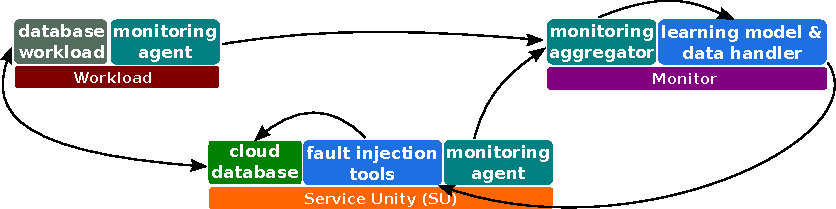
\includegraphics[width=1\textwidth]{inputs/img/roles_scheme}
  \caption{Main roles and interactions of Tejo prototype.}
  \label{fig:roles_scheme}
\end{figure}


\subsection{Installation}

In this subsection, we describe the main installation steps of our prototype. Our description will be based on the scheme depicted in Figure~\ref{fig:roles_scheme} and is organized as follows. First, we provide an overview of the installations tools available online. In turn, we describe the installation steps that are common to all roles. Then we describe installation steps that are specific to the roles, explaining the main steps to set-up a Monitor. After the Monitor set-up, we describe the installation of a SU and finally the installation of the Workload.

\subsubsection{Installation scripts and source code organization in the publicly available repository}
\label{subsubsec:gitclone}

All the scripts to perform the installation of the prototype of Tejo are available online~\footnote{An anomaly detection scheme for cloud databases: \url{https://github.com/guthemberg/tejo}}.  To start installing Tejo, retrieve the all sources from the online repository as follows:


\begin{lstlisting}
git clone https://github.com/guthemberg/tejo
\end{lstlisting}


Overall, the repository is organized in the following way.

\lstinputlisting[language=sh, firstline=1, lastline=22,frame=single]  {inputs/sources/repo_organization.txt}

There are two folders in the repository root: \verb|contrib| and \verb|tejo|. \verb|contrib| has a collection of scripts necessary to the installation procedure organized by operating system distribution and packages specificities. As we will explain in futher details in the following subsections, most of packages required to install our prototype are available on any unix-like system. However, for a matter of simplicity, we have adapted the installation scripts to be more comfortably performed in Debian systems, more precisely, to the 7.8 release. This includes all scripts and configuration files templates available inside \verb|contrib/debian|, which might be easily modified for other distributions. In \verb|contrib|, we provide a set of tools and templates to install Workload role in fedora-like systems, particularly customized for PlanetLab testbed. Moreover, one will find binaries of \verb|paping|~\footnote{paping: Cross-platform TCP port testing, emulating the functionality of ping (port ping). \url{https://code.google.com/p/paping/}}, a tcp-based tool for latency measurements, a template of the main configurations file of Tejo along with some of its miscellaneous/tuning scripts.

While \verb|contrib|  mostly provides installation scripts for third-party, required packages, \verb|tejo| has the main sources and modules of our prototype itself. It contains four directories: \verb|common|, \verb|data_handler|, \verb|fault_injection_tools|, and \verb|learning_model|. The first one has a collection of commonly performed tasks as Tejo runs, such as launching experiments and fault injection campaigns as well as monitoring database set-up scheme and backup. The latter three directories correspond pretty much to the modules described in Section~\ref{sec:design}. They actually provide the main functionalities of our prototype, including computing the monitoring data, fault injection campaign orchestration and learning/predictions of anomalies.

\subsubsection{Common installation steps}

Regardless the role of the node, we should perform a few preliminary installation steps to set-up Tejo. These steps mainly concern a set of common installation packages and some adjustments to configuration files. Table~\ref{tab:common_install_conf_node} concisely describes these steps and the configuration file templates to be customized.

			\begin{table*}[htdp]
				\begin{center}
\caption{Common required packages and main configuration file.}
  \label{tab:common_install_conf_node}
					\begin{tabular}{R{2.5cm} || L{4.5cm} L{6cm} }
						{\bf Requirement}&{\bf Template/packages}&{\bf Description} \\  
						\hline
						\hline
						{\bf Common packages}&rcconf sysv-rc-conf wget ntp ntpdate rdate screen htop apt-show-versions ethtool gcc git nmap less iperf bc tcsh & This list provides a common set of open-source packages required by the collection of Unix shell scripts of Tejo.\\
						\hline
						{\bf Python libraries/tools}&python-psutil python-pip python-configobj python-dev python-rrdtool python-psycopg2 & Most of scripts of Tejo are implemented in Python language, notably those that provide interface to database API, configuration file parsing, interface to monitoring data database API (rrd), etc.\\
						\hline
						{\bf Java}&openjdk-7-jdk & Several functionalities of Tejo require java (release 7 or higher) support, e.g. workload generator and query router/load balancer.\\
						\hline
						{\bf The main configuration file}&\verb|tejo/contrib/tejo/| \verb|tejo.conf.sample|&This file provides the main parameters for Tejo functioning and should be copied to \verb|/etc| directory. This file contains a couple of keywords in upper-case letters to be replaced/customized accordingly. At this point of the installation, the key words to be customized are: USER, GUEST\_PASSWORD, and MY\_DOMAIN.  \\
					\end{tabular}
				\end{center}
			\end{table*}



\subsubsection{Installing a Monitor node}

Monitor is the main role of Tejo prototype. As briefly described in Subsection~\ref{subsec:roles}, a node that plays this role is in charge of (i) aggregating and computing monitoring data, (ii) orchestrating fault injection campaigns and (iii) predicting anomalous behaviours. To do that, Tejo requires the installation of two additional packages and the customization of some configuration files. We provide a summary of these installation steps as follows.

			\begin{table*}[htdp]
				\begin{center}
\caption{Required packages and configuration file adjustments for a Monitor node.}
  \label{tab:common_install_conf}
					\begin{tabular}{R{2.5cm} || L{4.5cm} L{6cm} }
						{\bf Requirement}&{\bf Template/packages}&{\bf Description} \\  
						\hline
						\hline
						{\bf Postgres database}& postgresql, \verb|/contrib/debian/| \verb|pgsql/pg_hba.conf|& Tejo relies on a relational database scheme running on postgres to handle/maintain monitoring data. After postgres installation, we should be allowed to establish connections to the \verb|localhost|. To do that, replace the installed \verb|pg_hba.conf| by the one available in the retrieved repository.\\
						\hline
						{\bf Ganglia}&ganglia-monitor gmetad & Monitor nodes require the installation of ganglia system as poller and aggregator of monitoring data. To make ganglia work like that, two configuration files should be customized: \verb|tejo/contrib/debian/| \verb|ganglia/gmetad.conf.sample| and \verb|tejo/contrib/debian/| \verb|ganglia/gmond.conf.aggregator.sample|. These files contain two keywords (in upper-case letters) that should be replaced accordingly, namely TARGET and SOURCE. Further information about the configuration of ganglia are available online (Ganglia quick-start doc: \url{https://github.com/ganglia/monitor-core/wiki/Ganglia-Quick-Start}).\\
					\end{tabular}
				\end{center}
			\end{table*}

To accomplish the set-up of the postgres database of a Monitor role, we should recover a backup SQL scheme available in the repository.

\begin{lstlisting}
cp tejo/common/db/backups/monitor_001_pg_all_dbs_*_TEMPLATE.dump.gz \
	/tmp
su postgres -c "cd /tmp; \
	gunzip monitor_001_pg_all_dbs_*_TEMPLATE.dump.gz; \
	psql -f monitor_001_pg_all_dbs_*_TEMPLATE.dump postgres; \
	rm -rf monitor_001_pg_all_dbs_*_TEMPLATE.dump"
\end{lstlisting}

These commands allow us to set-up the PostgreSQL database with the scheme that Tejo will use. The template backup has no data, only the scheme is recovered.


\subsubsection{Installing a Service Unity node}
\label{subsubsec:su}

The Service Unity node is actually where runs the cloud database, whose cluster-based set-up is briefly described in Subsection~\ref{subsec:dbsetup}. Alongside the cloud database instance, there are fault injection tools and monitoring agent. While the fault injection tools allow us to emulate malfunctioning cloud infrastructure the monitoring agent collects a collection of measurements of the Service Unity node. The agent periodically sends these measurements to the monitor aggregator (as depicted in Fig.~\ref{fig:roles_scheme}). 

A Service Unity node requires minimal set-up. First, it is necessary to fetch sources, as described in \ref{subsubsec:gitclone}. The fault injection tools does not require any adjustment, since most of fault injection campaigns are launched remotely (further details in Subsection~\ref{subsec:conftejo}). The monitoring agent requires the following package:

			\begin{table*}[htdp]
				\begin{center}
\caption{Required packages and configuration file adjustments for a Service Unity node.}
  \label{tab:common_install_conf}
					\begin{tabular}{R{2.5cm} || L{4.5cm} L{6cm} }
						{\bf Requirement}&{\bf Template/packages}&{\bf Description} \\  
						\hline
						\hline
						{\bf Ganglia}&ganglia-modules-linux ganglia-monitor ganglia-monitor-python, \verb|/contrib/debian/| \verb|ganglia/gmond.conf.sample|, \verb|/contrib/debian/| \verb|ganglia/vm/*.py*| & Service Unity nodes require the installation of ganglia system as ``monitor'' or simply as an agent. For that, two categories of configuration files should be customized. The first category is the main configuration file which governs the behaviour of the ganglia monitor, whose a template is available in \verb|/contrib/debian/| \verb|ganglia/gmond.conf.sample|, to replace the original configuration file (that is the \verb|/etc/ganglia/gmond.conf| in Debian systems). The second category is a set of configuration files of additional plug-ins, available in \verb|/contrib/debian/| \verb|ganglia/vm/*.py*|. These plug-ins allow us to collect additional information about the node including metrics of the cloud database instance and fault campaign activity.\\
					\end{tabular}
				\end{center}
			\end{table*}


\subsubsection{Installing a Workload node}

To emulate the behaviour of requests from clients to the cloud database cluster, the Workload generates a number of requests to the cluster instances. In Tejo, the workload is emulate by YCSB, a benchmark for cloud services designed by Yahoo~\cite{cooper2010benchmarking}. Similar to fault injection tools, no additional set-up is required to YCSB, it makes part of Tejo sources, available online git repository. To accomplish the set-up of the Workload node, one should install and configure ganglia monitoring agent, detailed as follows: 

			\begin{table*}[htdp]
				\begin{center}
\caption{Required packages and configuration file adjustments for a Service Unity node.}
  \label{tab:common_install_conf}
					\begin{tabular}{R{2.5cm} || L{4.5cm} L{6cm} }
						{\bf Requirement}&{\bf Template/packages}&{\bf Description} \\  
						\hline
						\hline
						{\bf Ganglia}&ganglia-modules-linux ganglia-monitor ganglia-monitor-python, \verb|/contrib/debian/| \verb|ganglia/gmond.conf.sample|, \verb|/contrib/debian/| \verb|ganglia/wl/*.py*| & Similar to a Service Unity node, Workload ones require the installation of ganglia system as an agent and one might even use the same template for both type of node (as described in \ref{subsubsec:su} ). However, the files of additional plug-ins are different and should be copied from the Tejo installation directory \verb|/contrib/debian/| \verb|ganglia/wl/*.py*|. In fact, these files implement an additional plug-in for Workload nodes that collects measurements about the performance of YCSB, namely SLO metrics.\\
					\end{tabular}
				\end{center}
			\end{table*}



\subsection{Cloud database set-up}
\label{subsec:dbsetup}

In this section, we provide a brief overview of the main steps to install a cloud database cluster using MongoDB and VoltDB. The comprehensive documentation of MongoDB and VoltDB are available online~\footnote{MongoDB: https://docs.mongodb.org/manual/, VoltDB: http://docs.voltdb.com/}.

These distributed database systems provides two properties that are interesting to evaluate with Tejo: scalable and fault-tolerant data maintenance. They offer scalability by splitting data in L partitions or shards across a cluster of VMs. To increase the storage capacity of the cluster, operators may add nodes as the system run. To enhance data availability, data is replicated in K+1 copies, which allows the system to tolerate up to K VM failures. Depending on the scheme to maintain replicas, replication is divided in two broad groups: primary/secondary and multi-primary schemes. Essentially they differ on how requests that modify data are handled. Our approach takes into account both schemes. In addition, we assume that cloud database cluster rely on load balancing throughout replicas in order to limit the impact of cloud anomalies on a cluster.



\subsubsection{MongoDB}
\label{subsub:mongo}

Figure~\ref{fig:mongo_cluster} highlights the main components a MongoDB cluster and the interactions with the workload. There are two main components of a MongoDB cluster: mongos and mongod. mongos is the query router that receives requests and forwards them to nodes running mongod. Nodes running mongod actually maintains data and responds the requests. 

\begin{figure}[!h]
  \centering
     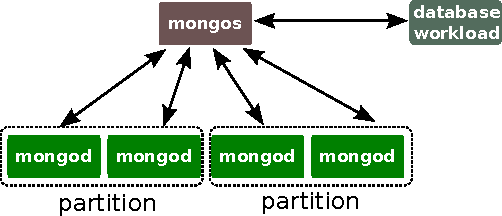
\includegraphics[width=.6\textwidth]{inputs/img/mongo_cluster}
  \caption{MongoDB cluster with five nodes, one query router (mongos) and four node replicas in two partitions (mongod).}
  \label{fig:mongo_cluster}
\end{figure}

The main packages and configuration files of MongoDB cluster are described a follows.

			\begin{table*}[htdp]
				\begin{center}
\caption{Required packages and configuration file adjustments for a Mongo.}
  \label{tab:common_install_conf}
					\begin{tabular}{R{2.5cm} || L{4.5cm} L{6cm} }
						{\bf Requirement}&{\bf Template/packages}&{\bf Description} \\  
						\hline
						\hline
						{\bf mongos}&\verb|/contrib/debian/mongodb/| \verb|install.sh|, \verb|/contrib/debian/mongodb/| \verb|etc/configdb/mongod.conf|, \verb|/contrib/debian/mongodb/| \verb|etc/qrouter/mongos.conf| & The mongos installation includes a script \verb|install.sh| and two configuration files. While the installation script install the main packages to run both the query router itself and the surrogate configuration daemon, the configuration files are specific to each one of them  and should be adjusted accordingly. \\
						\hline
						{\bf mongod}&\verb|/contrib/debian/mongodb/| \verb|install.sh|, \verb|/contrib/debian/mongodb/| \verb|etc/configdb/mongod.conf| & mongod installation and configuration are straightforward. Basically, the installation requires running the same script for mongos installation and the configuration requires he modification of the DBPATH configuration file variable.\\
					\end{tabular}
				\end{center}
			\end{table*}

Once mongos and mongod are installed and configured properly, the latest step is to add mongod instances to the mongos as follows:

\begin{lstlisting}
#once connected to the node running the mongos
sh.addShard( "rs0/primary-mongod-server-partition-0:27017, \
    rs1/primary-mongod-server-partition-1:27017" ) \
sh.shardCollection( "collection.name", 'key': { "_id": "hashed" } ) 
\end{lstlisting}

The first command adds the two primary copies to the query router (mongos) and the second creates a collection of documents whose storage are spread across the nodes according the hash value of the document keys. After set-upping and configuring the MongoDB cluster, we should load it with data. This step can be performed from the workload by running the following command:

\begin{lstlisting}
sh contrib/debian/mongodb/load.sh
\end{lstlisting}

This script loads a large number of documents into the database cluster. It uses the parameters of \verb|/contrib/debian/mongodb/ycsb-0.1.4/workloads/load|, which can be tuned for particular purposes. Finally, Tejo provides two scripts to run and stop the workload, namely \verb|/tejo/common/experiments_scripts/ycsb/run.sh| and \verb|/tejo/common/experiments_scripts/| \verb|ycsb/stop.sh|.


\subsubsection{VoltDB}

The set-up of a VoltDB cluster differs in two main points from that of MongoDB. First, there is no query router, the workload sends requests directly to nodes that maintain data. Second, its architecture is easier since there is no primary/secondary replica roles, resulting in a simpler deployment. Figure~\ref{fig:voltdb_cluster} depicts a simple VoltDB cluster with four replicas grouped in two partitions.

\begin{figure}[!h]
  \centering
     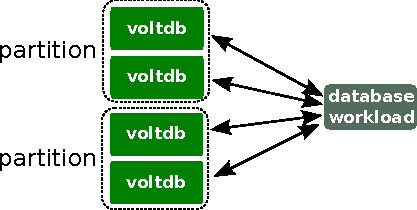
\includegraphics[width=.6\textwidth]{inputs/img/voltdb_cluster}
  \caption{VoltDB cluster with four nodes, four node replicas in two partitions.}
  \label{fig:voltdb_cluster}
\end{figure}

To install VoltDB, one might either clone VoltDB Community Edition from the public repository~\footnote{https://github.com/VoltDB/voltdb/} or download the Enterprise edition for trial~\footnote{http://learn.voltdb.com/DLSoftwareDownload.html}. We recommend the installation of the later because it includes key features such as high availability that are not currently available in the community edition.

One the VoltDB is installed in the cluster nodes, the database can be run from the Workload node using the following Tejo's scripts: \verb|/tejo/common/experiments_scripts/tpcc/run.sh| and \verb|/tejo/common/experiments_scripts/tpcc/stop.sh| to use a TPC-C workload~\footnote{http://www.tpc.org/tpcc/detail.asp}, and \verb|/tejo/| \verb|common/experiments_scripts/| \verb|voter-selfcheck/run.sh| and \verb|/tejo/| \verb|common/experiments_scripts/| \verb|voter-selfcheck/stop.sh| for another workload customized for VoltDB clusters.

\subsection{How to configure and use Tejo}
\label{subsec:conftejo}

The configuration and use of Tejo include the following steps: environment set-up, configuration file customization, running the workload and fault injection campaigns, and finally set-up learning/anomaly detection prediction. To illustrate the configuration and use of Tejo, this subsection is based on the deployment example depicted in Figure~\ref{fig:tejo_cluster}, which can be easily extended to larger deployments. As shown in this figure, we assume in this subsection the set-up of a MongoDB cluster with a query router and four data storage nodes as described in \ref{subsub:mongo}.

\begin{figure}[!h]
  \centering
     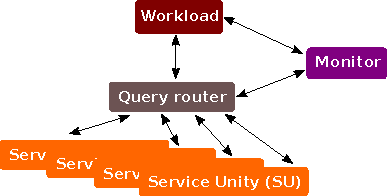
\includegraphics[width=.6\textwidth]{inputs/img/tejo_cluster}
  \caption{Tejo deployment.}
  \label{fig:tejo_cluster}
\end{figure}

\subsubsection{Environment set-up}

The Service Unity (SU) requires following packages to be installed on your local machine before configuration.

\begin{itemize}
	\item JDK/JRE +1.7~\footnote{http://www.ubuntuupdates.org/openjdk-7-jdk};
	\item Python +2.7~\footnote{http://www.ubuntuupdates.org/python};
	\item gcc/g++ +4.3~\footnote{http://www.ubuntuupdates.org/gcc};
	\item Ant +1.7~\footnote{http://www.ubuntuupdates.org/ant}.
\end{itemize}

In Debian systems, these packages can be installed by running the following packages:

\begin{lstlisting}
sudo apt-get -q -y update 
sudo apt-get -q -y  install git gcc g++ openjdk-7-jdk ant
\end{lstlisting}

In addition to these required packages, nodes in Tejo should be able to communicate directly through OpenSSH without password. First, you should install and set-up a public-private dsa key pair in the Monitoring node as follows:

\begin{lstlisting}
sudo apt-get -q -y install openssh-server
ssh-keygen -t dsa # Please do not enter in a password
cat ~/.ssh/id_dsa.pub >> ~/.ssh/authorized_keys
\end{lstlisting}

Then, we should performing the following steps in the remaining nodes, including SUs and Workload nodes.

\begin{lstlisting}
sudo apt-get -q -y install openssh-server
cat ~/.ssh/id_dsa.pub >> ~/.ssh/authorized_keys
\end{lstlisting}
where \verb|~/.ssh/id_dsa.pub| is the same file initially generated in the Monitor node.
 
\subsubsection{Configuration file}

The file \verb|/etc/tejo.conf| is the main configuration file of Tejo and it should be installed and tuned on each node properly. By cloning the sources from the public repository (described in \ref{subsubsec:gitclone}), you will download a template file whose some parameter key should be changed accordingly.

To install the template, run:
\begin{lstlisting}
cp tejo/contrib/tejo/tejo.conf.sample /etc/tejo.conf
\end{lstlisting}

The key parameters to be tuned are:

			\begin{table*}[htdp]
				\begin{center}
\caption{Key parameters of /etc/tejo.conf.}
  \label{tab:common_install_conf}
					\begin{tabular}{R{4cm} || L{6cm} L{3cm} }
						{\bf Parameter}&{\bf Description}&{\bf Examples} \\  
						\hline
						\hline
						{\bf node\_type}&It specifies the role of the node. The possible strings are vm (for SU), monitor, and workload & node\_type=monitor. \\
						\hline
						{\bf location}&This is a parameter that allows Tejo to identify the geographical location of a node. One might set ant string to this parameter. & location=eu, for nodes deployed on European datacenters. \\
						\hline
						{\bf rrd\_path\_vms\_prefix} and {\bf rrd\_path\_workload \_hosts\_prefix}&These are paths to rrd files and should be set only for nodes playing a Monitor role. This path is specific to the operating system. & /var/lib/ganglia/rrds/workload. \\
						\hline
						{\bf guest\_vm\_sys\_user} &Local system user who will deploy and run Tejo.&guest\_vm\_sys\_user= guest\\
						\hline
						{\bf root\_dir} &Path towards which Tejo will be cloned. It is usually the home directory of a system user.&root\_dir= /home/guest\\
						\hline
						{\bf home\_dir} &Destination path of local Tejo repository cloned copy. It is usually inside the home directory of a system user.&home\_dir= /home/guest/tejo\\
						\hline
						{\bf mongo\_query\_ router\_host} &Hostname of the query router.&mongo\_query\_ router\_host= FQDN.of.qrouter\\
						\hline
						{\bf system\_id} &This parameter is specific to the Workload node and describes which kind of systems it is querying.&system\_id= 0, for MongoDB read-only workload, 1 for VoltDB TPC-C, 2 for MongoDB reads and updated, and 3 for VoltDB voter workload.\\
					\end{tabular}
				\end{center}
			\end{table*}

\subsubsection{Workload and fault injection campaigns}

Once the nodes are set-up and configured properly, Tejo provides scripts to run workloads and fault injection campaigns that are easy to perform.

To run a workload, one should run the following script from the Workload node.

\begin{lstlisting}
sh tejo/tejo/common/experiments_scripts/quick_launch/run.sh
\end{lstlisting}

this launches requests to SUs. Then, you can launch a fault campaign from the Monitor node as follows.

\begin{lstlisting}
sh tejo/tejo/common/experiments_scripts/quick_launch/inject.sh
\end{lstlisting}

this scripts remotely injects faults in SUs. Finally, to stop the launched workload, run the following script from the Workload node:

\begin{lstlisting}
sh tejo/tejo/common/experiments_scripts/quick_launch/stop.sh
\end{lstlisting}

\subsubsection{Set-up learning and anomaly prediction}

The set-up of Tejo for learning and predicting has two major steps: periodic collection of measurements and data analysis.

The collection of measurements can be performed periodically using the \verb|crontab| of the Monitor node as follows:
\begin{lstlisting}
crontab  -r #to erase the previous jobs
crontab  tejo/data_handler/cron.job
\end{lstlisting}

these commands allow us to read rrd files and store them into the PostgreSQL database periodically.

For data analysis, data should be carefully selected from the database, preprocessed and finally put into the learning scripts. as selecting raw data, one should get data from two main tables of the PostgreSQL database, namely vm and slo. The following example shows a query template for doing that:

\begin{lstlisting}
select \$list\_of\_columns from vm inner join slo on slo.ts=vm.ts where \$filters order by vm.ts
\end{lstlisting}

This query template defines a aggregated list of comma-separated columns ,\$list\_of\_columns (about 200 columns, including SU/vm resources consumption, slo performance from the workload, and fault injection activity), selected from a join sql command over the two main tables, vm and slo. \$filters defines the restrictions of our query, mainly concerning the time-stamp column and and fault injection activity.

Once the raw data is collected and stored to a a file (either binary like pickle python os cvs-based text file), you can start preprocessing this data. Preprocessing the raw selected data is very simple and essentially consists in attributing labels to selected lines. Labels definition depends on the learning/prediction tasks. For example, if the goal is distinguish faulty from faulty-free nodes, just two labels are required, e.g. -1 for faulty SU nodes and 1 otherwise.

The latest step of the learning/prediction step is to feed the preprocessed data to the learning script. To this aim, Tejos provides a straightforward, easy-to-customize python script, which contains the definition of a supervised-learning classifier. This file is available on the following Tejo repository path:

\begin{lstlisting}
tejo/learning_model/anomaly_detection.py
\end{lstlisting}

it defines a anomaly detection classifier whose python class is called \verb|OneClassSVMClassifier|. This class is based on Scikit Learning~\footnote{http://scikit-learn.org/}, an open-source machine learning library, and implements two methods for anomaly detection: the instantiation and the predict method. The former allows us to read the preprocessed file (the training dataset), interpret the attributed labels, and learning anomalous behaviour of faulty nodes. This initial learning phase is run in batch mode. The second, the predict method, can be run on real deployments to predict anomalous SUs. 